%!TEX root = ../crimson_throne_book_main.tex
% 2016-03-05
The party slips away from the market district before the orc guards notice them. Some passers-by definitely recognize Sjo and Balian for humans, but since they are still in a 'pinkskin-allowed' zone, their presence does not immediately raise suspicion. Making their way down a street in the direction of the temple district, the heroes resume their search for a hide-out for the night. Quint spots a ruined building in a street that veers off to the left. A recent earthquake took the house down, taking its now half-rotted owner with it. There are signs that the place was plundered afterwards, which comes as no surprise in this inhospitable orc city. The back kitchen of the building miraculously survived the quake and is still standing. Its door has been kicked in, but enough of it remains to block the bottom half of the entrance. The companions take refuge in the ruined room and rest up, making sure to keep watch all night.\\

\section{19 Arodus 4708}

It is still early in the morning when the party members have regained their energy and spells and leave for the temple district. At this hour of day (or rather night) the city seems to be at its quietest. Quint uses his make-up skills to give everyone a half-orc appearance. Although it will probably not pass scrutiny, it might suffice to fool anyone who casually glances at the heroes. Following the directions they received yesterday, the companions find a broad lane that leads them out of the tunnels to a grand square. The first rays of the sun light an impressive cathedral, obviously a feat of dwarven architecture. The massive building of marble stone rises over a hundred feet into the air. Still, orc interference has had its effect: rusted metal plates with spikes and barbed spears adorn the front of the temple. The walls above these plates bear crude paintings of orcs in battle. Various statues have been defiled and remodeled to look like orcs or vile beasts. A broad set of stairs provides access to the immense front doors. Six orc soldiers stand at attention at the entrance.\\

Checking the map in the spy's notes again, the companions figure out that they have to get to the back of the temple. Keeping to the far edge of the square, the party circles the cathedral, easily making it to the other side. The focal point of a smaller square at the back side of the temple is a large fountain that must have been beautiful once. Various animals and creatures of stone lie at the feet of three central statues. These one-time dwarven heroes have been resculpted into hideous orcs. A dozen spouts spew out reddish-brown water that smells of rust and sewage. Fortunately this corner of the city is quiet at this time of day. Puk jumps over the statues to the central figures and starts looking for a secret door. Quint joins him, but their first quick search does not reveal anything. Then Puk gets into a dwarven mindset. Where would he hide a secret mechanism if he was a dwarf? A burrowing animal perhaps? Checking the different animal statues, the halfling discovers a small mole figure. When he presses the blind creature's eyes simultaneously, a slab of stone behind the central sculptures slides up. Squeezing between the statues and the wall, the heroes reach the entrance, which leads down into the dark.\\

The stairs take the companions to a\hyperref[fig:Urgir-tomb-Level-1-594710874]{ small dwarven crypt } . Quint casts  {\itshape light} on a coin to allow the party to see. All the graves have been plundered a long time ago; only broken stone, dust and bones remain. A second set of stairs in the center of the room leads further down. Puk's keen ears pick up orc voices from below. Quint performs a round of  {\itshape heroism} on the party before they dive deeper into the earth. \hyperref[fig:Urgir-tomb-Level-2-594712324]{ A second, slightly bigger crypt holds a troop of ten orcs, half of whom carry an axe, the other five wield swords. } Sjo opens combat with a  {\itshape fireball} , while Quint casts  {\itshape haste} and starts  {\itshape satire} to debuff the enemies. Balian swings his greatsword with great fervor, cutting down one orc in the first moments of combat. He forms a line with Puk to shield his friends, but the two of them get completely surrounded by enemies. Spyder blocks off another orc who tries to circle around the back pillar of the room. Sjo calls forth a  {\itshape prayer} to aid his friends and debuff the orcs even more, while Quint summons six  {\itshape mirror images} and draws his blade to assist Spyder. Balian and Puk take down two more orcs, but the ranger suffers some grievous wounds himself and requires healing. Sjo jumps to the rescue, giving Balian enough breath to cut down another orc with one mighty blow. The healer is now in the thick of battle as well and gets dealt a bloody cut. Puk and Balian push the attack and skewer two more opponents. Still the remaining orcs show no sign of backing down, dealing a few more wounds before they too fall to the heroes' weapons. After patching themselves up and storing some loot in their  {\itshape bag of holding} , the companions take a spiral staircase that descends even deeper in the earth. \\

\begin{figure}[h]
	\centering
	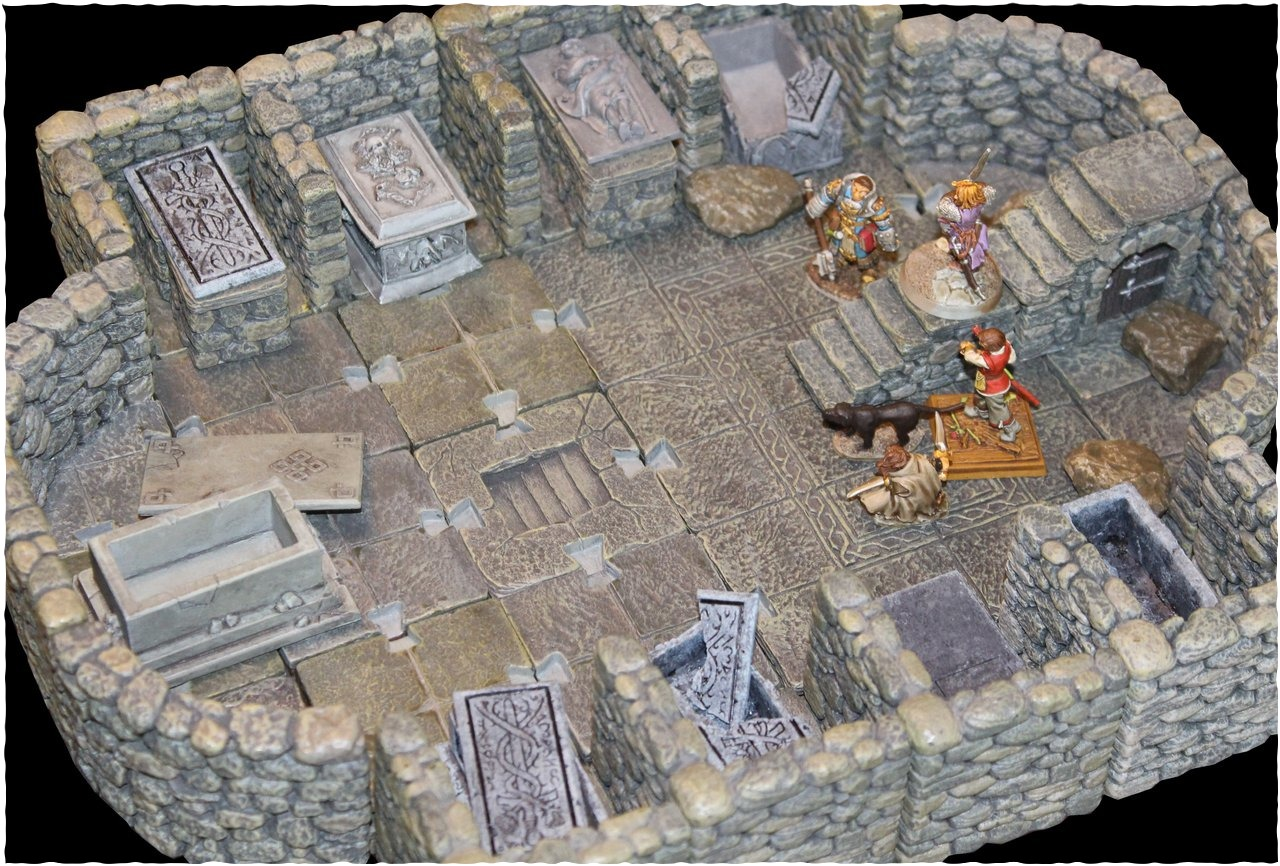
\includegraphics[width=0.4\textwidth]{images/Urgir-tomb-Level-1-594710874_mod.jpg}
	\caption{Urgir tomb Level 1}
	\label{fig:Urgir-tomb-Level-1-594710874}
\end{figure}

\begin{figure}[h]
	\centering
	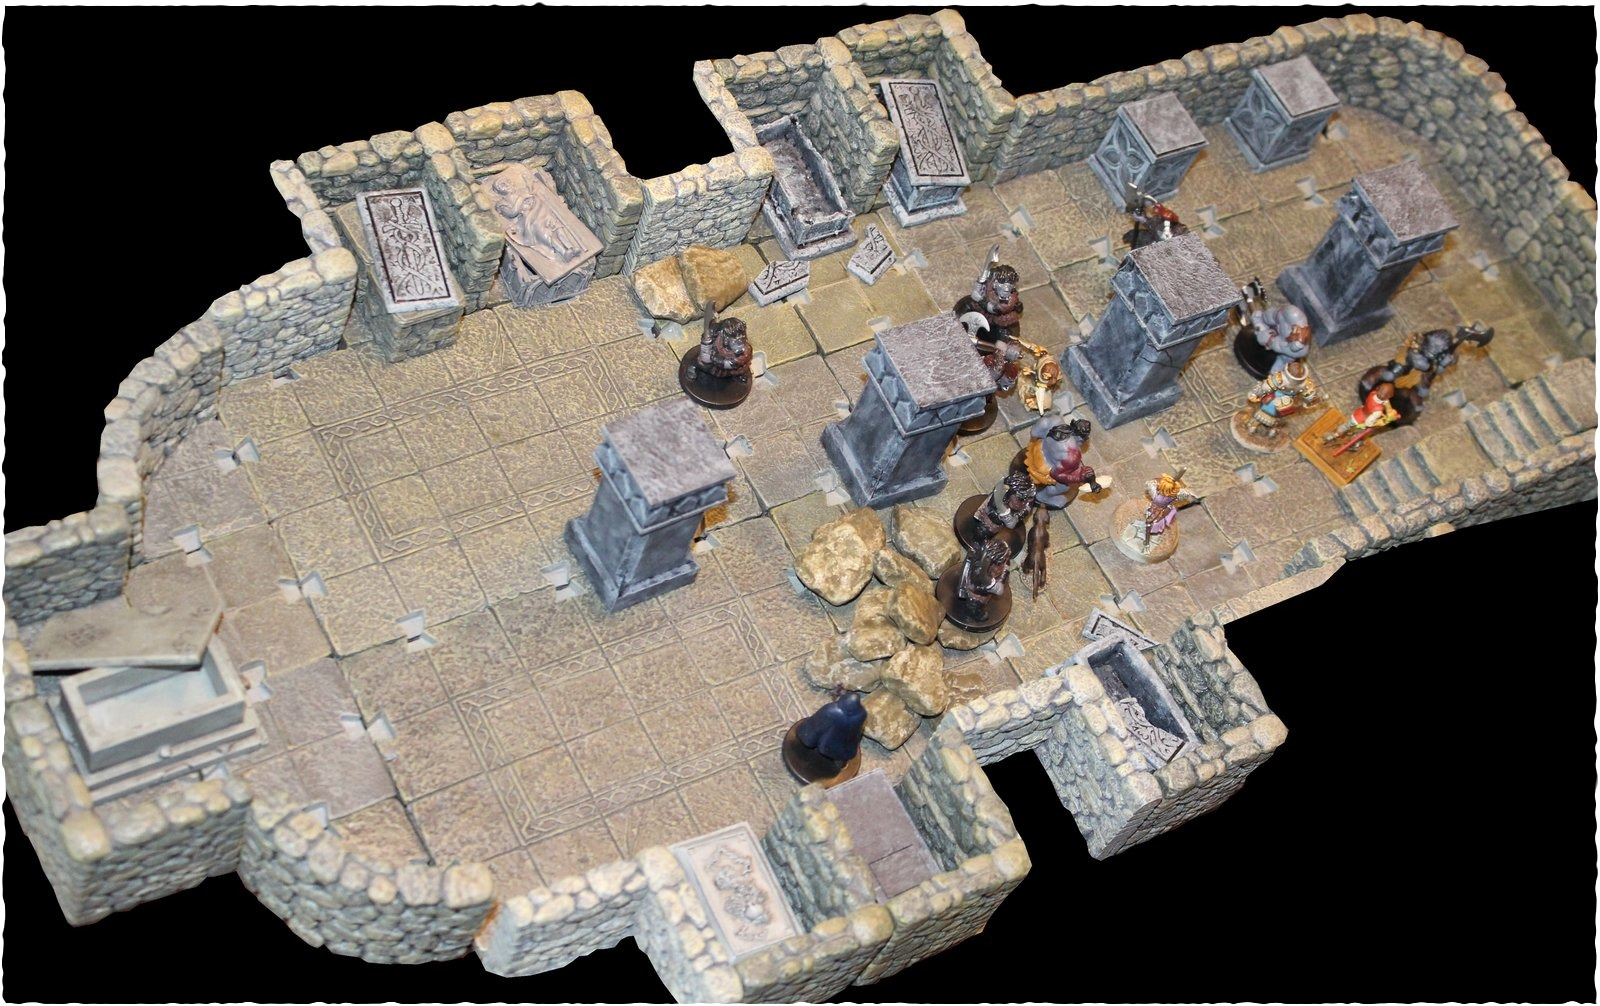
\includegraphics[width=0.4\textwidth]{images/Urgir-tomb-Level-2-594712324_mod.jpg}
	\caption{Urgir tomb Level 2}
	\label{fig:Urgir-tomb-Level-2-594712324}
\end{figure}

Once more Puk hears the sound of orcs grunting and arguing below. Sjo fears the rattling of his heavy plate will give him away and enspells a coin with {\itshape silence} , so he can move down unheard. The heroes reach a third, even larger crypt where they spot some light coming from behind the corner. Puk scouts ahead and sees four orcs down the hall. Quint decides to pull them in and uses  {\itshape ghost sound} to simulate the noise of a skeleton rising in one of the plundered tombs. The orcs take a few moments before they move in to explore. Puk, who is hiding behind a pillar near the orcs, hears someone casting a few spells first and someone else starting a bardic song of inspiration. When the orcs storm past, the halfling stabs one of them in the back, continuing his attacks until the creature goes down. Quint casts  {\itshape haste} on the party, but notices that the orcs have been similarly enhanced. \hyperref[fig:Urgir-tomb-Level-3-594713616]{ An axe-wielding orc bears down on Puk now and delivers a tremendous blow. } Sjo attacks the orc fighter, while Quint lashes out with his whip and trips one of the orc rogues. The creature gets back up quickly, suffering two attacks of opportunity from Balian and Spyder in the process, but in turn he gives the ranger a vicious cut as well. Puk realizes that the three remaining orcs he and his friends are currently targeting are nothing but cannon fodder for two invisible casters who are coming up from deeper in the crypt. One caster's  {\itshape slow} spell lifts both his and Spyder's  {\itshape haste} , while the other one keeps bolstering the skirmishing orcs with his song. Once more the axe-wielder hits the halfling with incredible strength, knocking the unfortunate halfling unconscious. The creature continues his attacks on Sjo and survives Quint's trip attempt. Spyder senses that one of the invisible casters has crawled up close and suddenly sees how a  {\itshape cone of cold} seems to appear out of thin air, catching all standing heroes in its blast. The orc rogue backstabs Sjo and the healer goes down as well. Balian stands the hero and cuts down the visible orcs in quick succession, but gets covered in  {\itshape glitterdust} by one of the casters and cannot see anything anymore as a result. A moment later three  {\itshape scorching rays} take the ranger out, while one of the invisible attackers -- the singing bard -- now targets Spyder with his blade. Although the dog smells where the assailant is, it does not succeed in biting him. Quint hides behind one of the pillars around the corner and casts  {\itshape mirror image} on himself, while the unseen bard presses the attack on Spyder and defeats the dogs as well. Four down, one to go! Now where is that annoying human bard hiding? \\

\begin{figure}[h]
	\centering
	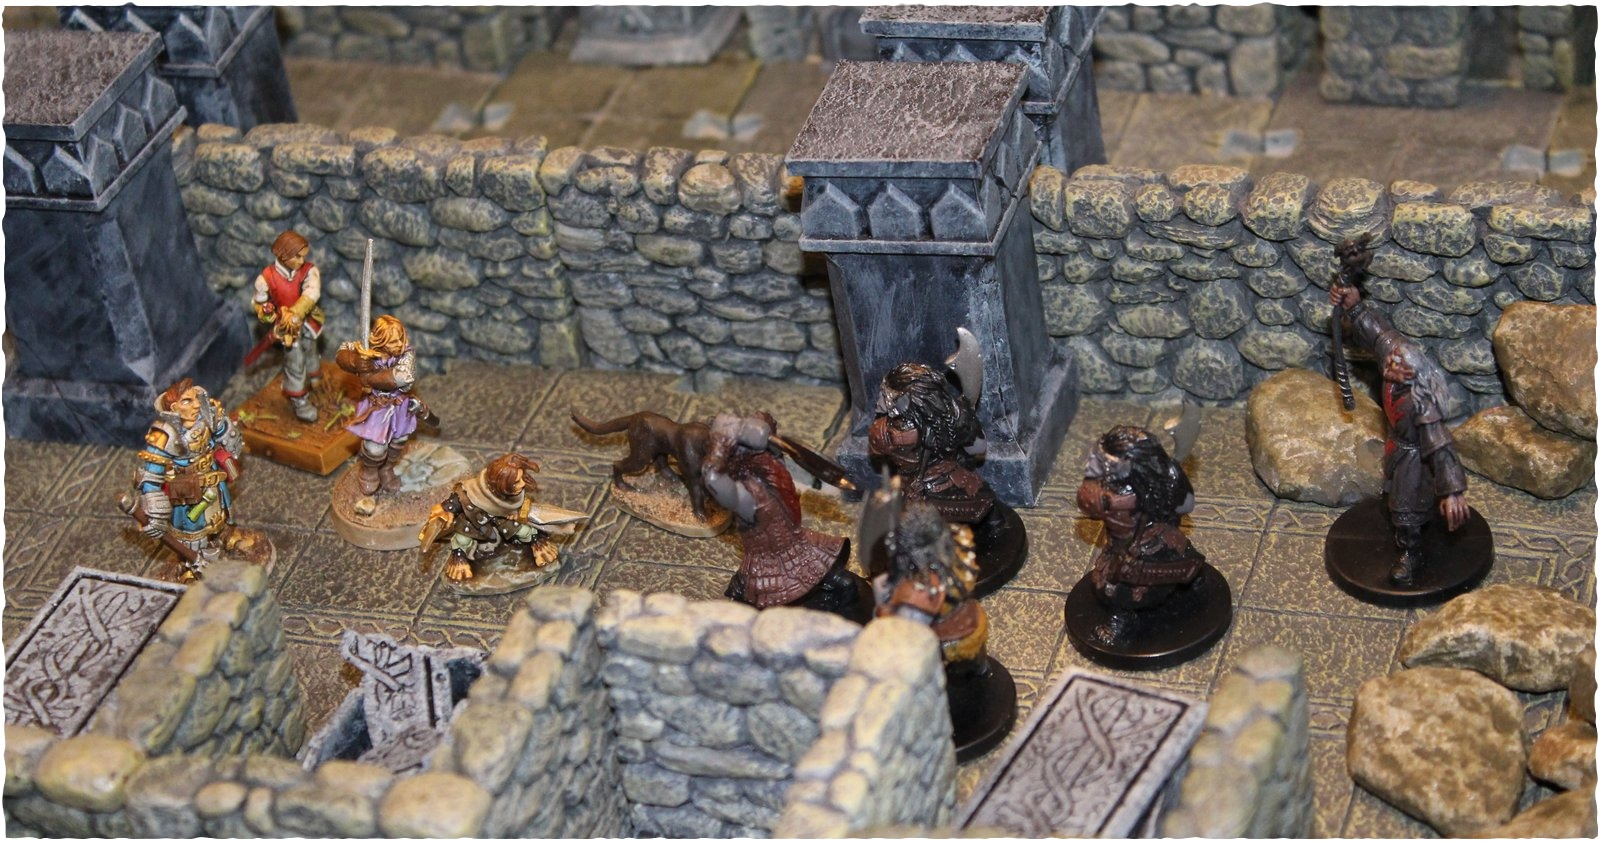
\includegraphics[width=0.4\textwidth]{images/Urgir-tomb-Level-3-594713616_mod.jpg}
	\caption{Urgir tomb Level 3}
	\label{fig:Urgir-tomb-Level-3-594713616}
\end{figure}

This is where we left the session, everyone in the party has been knocked into their negatives, except for Quint, who is tucked away behind a pillar around the corner. Two powerful casters, hiding under the cloak of 